\documentclass{article}
\usepackage[T1]{fontenc}
\usepackage[utf8]{inputenc}
\usepackage{anysize}
\marginsize{2.5cm}{2.5cm}{1cm}{1.5cm}
\usepackage{amsmath} %koniecznie
\usepackage{amssymb,amsfonts,amsthm}%dodatkowo
\usepackage{tikz}
\usepackage{pgfplots}
\usepackage{gensymb}
\usepackage{polski}


\title{Fizyka dla Informatyków, wykład\\ Sprawozdanie z realizacji zadania zespołowego programistycznego}
\author{Jan Bylicki \and Jan Chlebek \and Ryszard Dotka \and Marcin Kasznia}
\date{31 sierpnia 2020}

\begin{document}

\maketitle

\section{Wstęp}
Zadanie programistyczne zrealizowano w wariancie B tj. dotyczącym symulacji dwuwymiarowego gazu. Do implementacji wykorzystano język \verb+Python 3.8+ (jednak nie wykorzystywano elementów dodanych w najnowszych wersjach, zatem program powinien z powodzeniem działać na starszych wersjach interpretera). Działanie programu przetestowano pod kontrolą systemu operacyjnego \verb+Ubuntu 20.04.1 LTS x86_64+, \verb+Manjaro Linux kernel 5.4.57 x86_64+ oraz \verb+Windows 10+. Posłużono się niektórymi technikami programowania obiektowego. Program wyposażono w okno graficzne, prezentujące aktualny stan symulacji, umożliwiające zmianę upływu czasu (pauza, cofanie, krok o jedną klatkę), informacje o upływie czasu (liczby klatek) oraz wykres prezentujący w zależności od czasu drogę przebytą przez czerwony atom od ostatniego zderzenia.\\
Program składa się z wielu plików, a jego uruchomienie następuje poprzez plik \verb+main.py+. Po uruchomieniu programu można wprowadzić argumenty symulacji, w przypadku ich pominięcia przyjęte zostaną warotści domyślne.
W dalszej części sprawozdania przedstawiono informacje formalne oraz prezentacje przeprowadzonych pomiarów.

\section{Skład zespołu}
Zadanie zostalo zrealizowane w zespole o następującym składzie:
\begin{enumerate}
    \item Jan Bylicki (I4.1; 145441; jan.bylicki@student.put.poznan.pl)
    \item Jan Chlebek (I4.1; 145380; jan.chlebek@student.put.poznan.pl)
    \item Ryszard Dotka (I4.1, 145305; ryszard.dotka@student.put.poznan.pl)
    \item Marcin Kasznia (I5.1; 145379; marcin.kasznia@student.put.poznan.pl)
\end{enumerate}

\section{Wykaz prac wykonanych przez członków zespołu}
    \subsection{Jan Bylicki}
        Implementacja warstwy graficznej symulacji (część funkcji w klasie \verb+Box+, funkcja \verb+main_loop+ w pliku \verb+main.py+) oraz zapisu stanu symulacji (plik \verb+cache+)
    \subsection{Jan Chlebek}
        Pomysł i implementacja algorytmu generującego stan początkowy (tak aby nie powstawały kolizje). Wsparcie przy towrzeniu silnika matematycznego. Implementacja skryptu generującego wyniki symulacji do pliku tekstowego. Przygotowanie sprawozdania z projektu.
    \subsection{Ryszard Dotka}
        Implementacja kodu odpowiedzialnego za sterowanie przepływem symulacji (pauza, praca krokowa, cofanie) łącznie z warstwą graficzną (plik \verb+control.py+). Implementacja funkcji odpowiadających za rozpoczęcie programu (plik \verb+setup.py+). Przygotowanie i przeprowadzenie pomiarów.
    \subsection{Marcin Kasznia}
        Implementacja następujących klas: \verb+Box+, \verb+atom+, \verb+red_atom+, odpowiadających za silnik matematyczno-fizyczny symulacji. Wsparcie techniczne (\LaTeX) przy przygotowaniu sprawozdania.

\section{Procentowy udział w realizacji projektu członków zespołu}
\begin{enumerate}
    \item Jan Bylicki: 25\%
    \item Jan Chlebek: 25\%
    \item Ryszard Dotka: 25\%
    \item Marcin Kasznia: 25\%
\end{enumerate}
\section{Wykaz przesłanych plików}
    Kod źródłowy programu: \verb+Source_145380.zip+ zawierający:
    \begin{enumerate}
        \item Program główny: \verb+main.py+
        \item Definicja klasy \verb+Box+: \verb+box.py+
        \item Definicje klas \verb+atom+ i \verb+red_atom+: \verb+atom.py+
        \item Obsługę zarejestrowanego stanu symulacji: \verb+cache.py+
        \item Obsługę wyników symulacji: \verb+export.py+
        \item Definicje klasy \verb+Graph+ (odpowiedzialnej za wykresy wewnątrz symulacji): \verb+graph.py+
        \item Definicje klas \verb+Button+ i \verb+Slider+: \verb+control.py+
        \item Zbiór zmiennych dotyczących układu symulacji: \verb+layout.py+
        \item Zewnętrzną bibliotekę graficzną: \verb+graphics.py+
        \item Wyniki uzyskane w symulacji: katalog \verb+report+ zawierający:
        \begin{itemize}
            \item Skrypt zbierający dane: \verb+results.py+
            \item Wyniki otrzymane z pomiarów: \verb+results.csv+
            \item Plik źródłowy sprawozdania w formacie \LaTeX: \verb+report.tex+
            \item Zrzuty ekranu: \verb+Screenshot X.png+
        \end{itemize}
    \end{enumerate}
\section{Wykaz zapożyczonych bibliotek}
W projekcie wykorzystano następujące zewnętrzne biblioteki (jeżeli nie wskazano inaczej pochodzą one ze standardowej instalacji interpretera języka Python lub oficjalnych repozytoriów PyPI):
    \begin{enumerate}
        \item \verb+graphics.py+ (załączono całość kodu źródłowego) źródło: John M. Zelle \verb+mcsp.wartburg.edu/zelle/python/+
        \item \verb+tkinter+
        \item \verb+numpy+
        \item \verb+copy+
        \item \verb+time+
        \item \verb+math+
        \item \verb+os+
        \item \verb+random+
        \item \verb+sys+
    \end{enumerate}
\section{Zrzuty ekranowe ilustrujące działanie programu}
    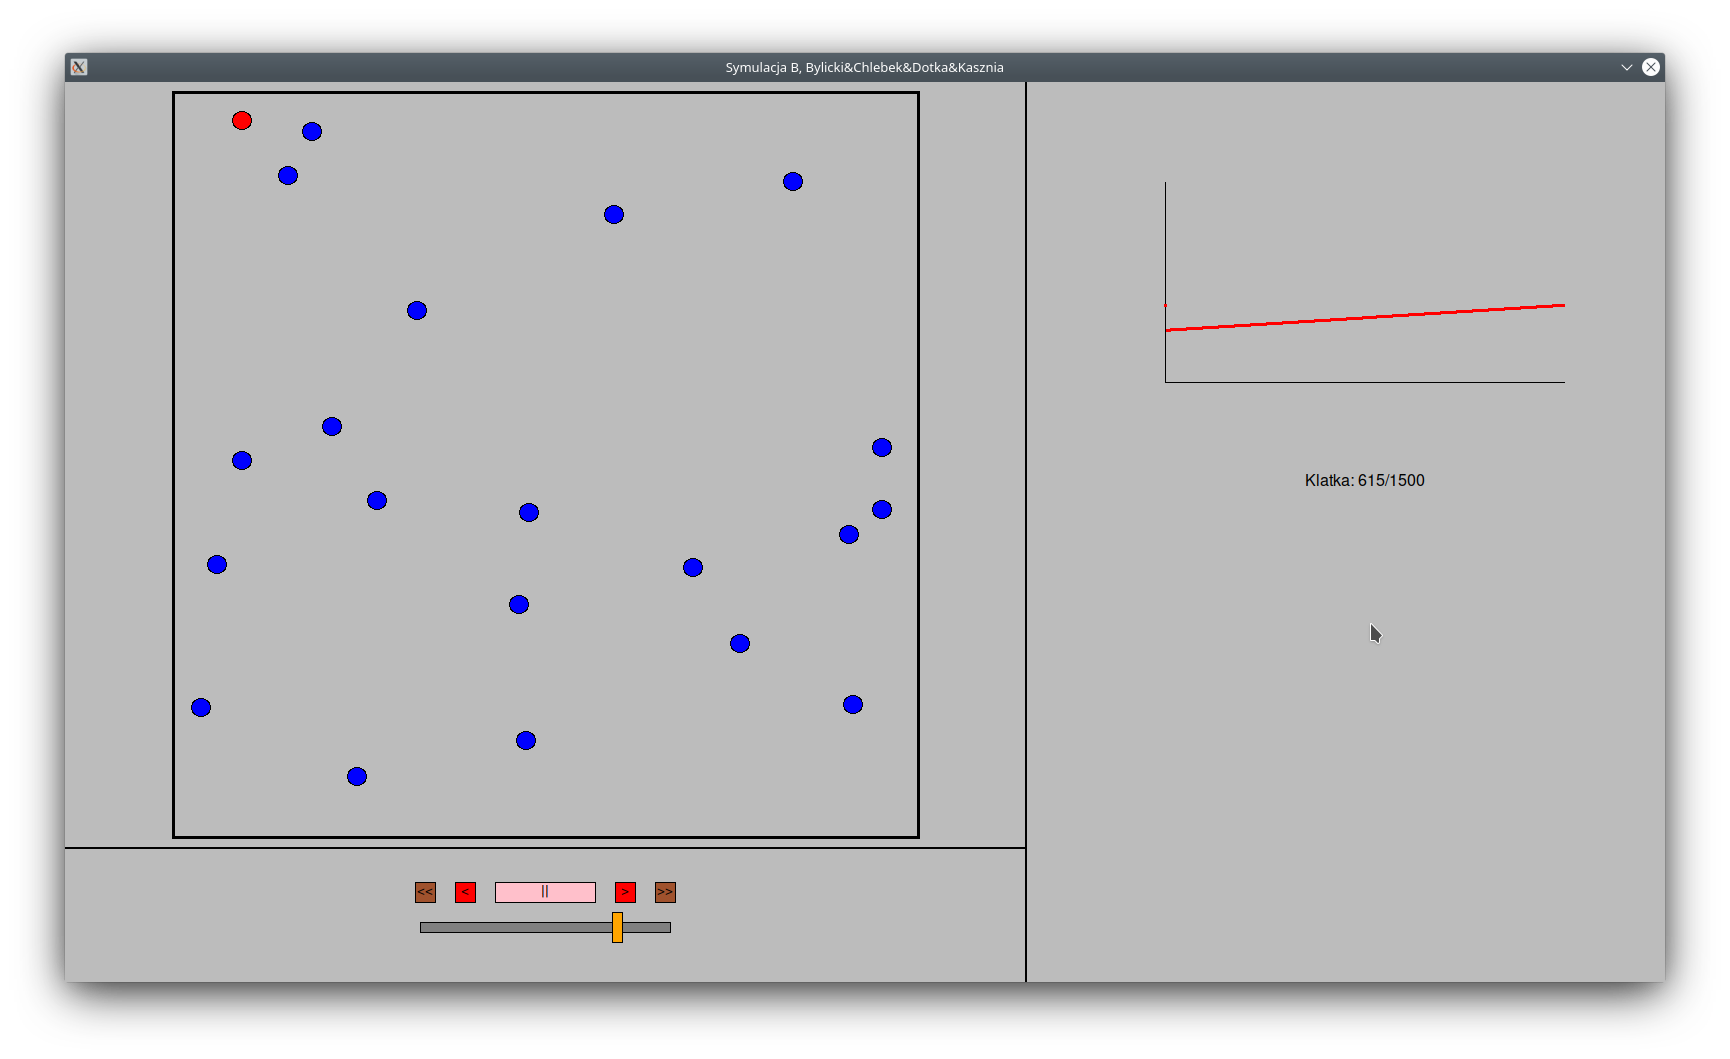
\includegraphics[width=\textwidth]{Screenshot 1.png}\\
    
    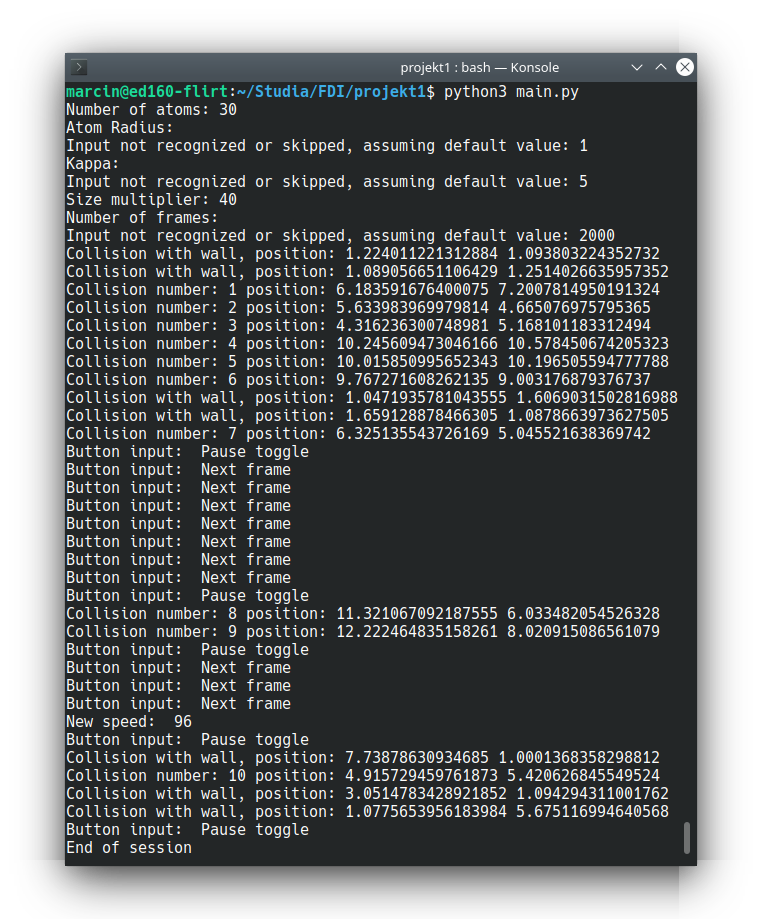
\includegraphics[width=\textwidth]{Screenshot 2b.png}\\
\section{Wykresy}
Na poniższych wykresach przedstawiono zgodnie z poleceniem średnią odległość przebytą przez czerwony atom między zderzeniami i liczbę tych zderzeń w zależności od liczby atomów w pojemniku, dla różnych czasów trwania (liczby klatek) symulacji.\\
Pomiary przeprowadzono dla następujących wartości startowych:
\begin{itemize}
    \item Liczba atomów: $n\in\{10,20, 30, 40, 50, 60, 70, 80, 90, 100\}$
    \item Promień atomów: $r=1$
    \item $\kappa=5$
    \item Współczynnik wielkości pojemnika: $\eta=50$
    \item Liczba klatek: $M \in \{500, 1000, 1500\}$
\end{itemize}
W trakcie testów programu wybrano wartość $\kappa=5$ jako dającą oczekiwane rezultaty w kontekście dokładności oraz szybkości działania programu.\\
\begin{center}
    \begin{tikzpicture}[scale=1]
        \begin{axis}[
        xlabel={Liczba atomów},
        ylabel={Średnia droga między zderzeniami},
        %xmin=0,xmax=5500,
        %ymin=0,%ymax=0.0105,
        scale=1.4,
        legend pos=north east,
        ymajorgrids=true,grid style=dashed
        ]
        
        \addplot[color=blue,mark=square] %500
        coordinates {
            % (10,80.2307614867876)
            (20,12.4855115050347)
            (30,13.3271684335507)
            (40,15.3187389301808)
            (50,5.17939606961693)
            (60,4.77245146911994)
            (70,8.46422829646755)
            (80,4.82567600345608)
            (90,2.62268538953038)
            (100,2.94642267143884)
        };
        
        \addplot[color=green,mark=square] %1000
        coordinates {
            (10,20.7939677742379)
            (20,15.7719462396346)
            (30,12.1090745762175)
            (40,10.459172180169)
            (50,6.75777136277276)
            (60,5.87356487503462)
            (70,7.46606345850943)
            (80,2.8278517840436)
            (90,4.02938051000513)
            (100,2.55368546693458)
        };
        
        \addplot[color=red,mark=square] %1500
        coordinates {
            (10,24.4724031317112)
            (20,18.6706536290102)
            (30,10.5719267598507)
            (40,11.0527730797002)
            (50,6.59623906431116)
            (60,6.16342283639367)
            (70,4.81262460308959)
            (80,2.25532970958734)
            (90,1.39945262690461)
            (100,3.35242426128515)
        };
       
        \legend{500 klatek,1000 klatek,1500 klatek}
        \end{axis}
    \end{tikzpicture}
\end{center}

\begin{center}
    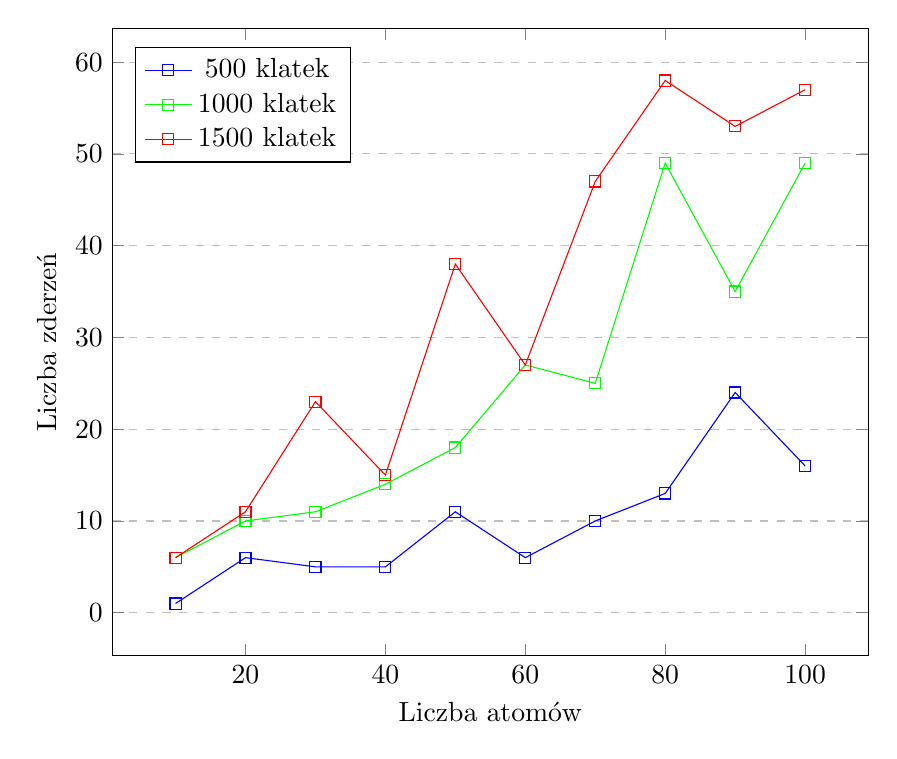
\begin{tikzpicture}[scale=1]
        \begin{axis}[
        xlabel={Liczba atomów},
        ylabel={Liczba zderzeń},
        %xmin=0,xmax=5500,
        %ymin=0,%ymax=0.0105,
        scale=1.4,
        legend pos=north west,
        ymajorgrids=true,grid style=dashed
        ]
        
        \addplot[color=blue,mark=square] %500
        coordinates {
            (10,1)
            (20,6)
            (30,5)
            (40,5)
            (50,11)
            (60,6)
            (70,10)
            (80,13)
            (90,24)
            (100,16)
        };
        
       \addplot[color=green,mark=square] %1000
        coordinates {
            (10,6)
            (20,10)
            (30,11)
            (40,14)
            (50,18)
            (60,27)
            (70,25)
            (80,49)
            (90,35)
            (100,49)
        };
        
        \addplot[color=red,mark=square] %1500
        coordinates {
            (10,6)
            (20,11)
            (30,23)
            (40,15)
            (50,38)
            (60,27)
            (70,47)
            (80,58)
            (90,53)
            (100,57)
        };
        
        \legend{500 klatek,1000 klatek,1500 klatek}
        \end{axis}
    \end{tikzpicture}
\end{center}
Na podstawie uzyskanych wyników można stwierdzić, że wraz ze wzrostem liczby atomów w pudełku (gęstości) spada średnia odległość pomiędzy kolejnymi zderzeniami. Jednocześnie liczba tych zderzeń w jednakowej jednostce czasu rośnie.
\end{document}
